\documentclass[
  bibliography=totoc,     % Literatur im Inhaltsverzeichnis
  captions=tableheading,  % Tabellenüberschriften
  titlepage=firstiscover, % Titelseite ist Deckblatt
  parskip=half,           % schöner Zeilenabstand
]{scrartcl}

% Paket float verbessern
\usepackage{scrhack}

% Warnung, falls nochmal kompiliert werden muss
\usepackage[aux]{rerunfilecheck}

% unverzichtbare Mathe-Befehle
\usepackage{amsmath}
% viele Mathe-Symbole
\usepackage{amssymb}
% Erweiterungen für amsmath
\usepackage{mathtools}

% Fonteinstellungen
\usepackage{fontspec}
% Latin Modern Fonts werden automatisch geladen
% Alternativ zum Beispiel:
%\setromanfont{Libertinus Serif}
%\setsansfont{Libertinus Sans}
%\setmonofont{Libertinus Mono}

% Wenn man andere Schriftarten gesetzt hat,
% sollte man das Seiten-Layout neu berechnen lassen
\recalctypearea{}

% deutsche Spracheinstellungen
\usepackage{polyglossia}
\setmainlanguage{german}


\usepackage[
  math-style=ISO,    % ┐
  bold-style=ISO,    % │
  sans-style=italic, % │ ISO-Standard folgen
  nabla=upright,     % │
  partial=upright,   % ┘
  warnings-off={           % ┐
    mathtools-colon,       % │ unnötige Warnungen ausschalten
    mathtools-overbracket, % │
  },                       % ┘
]{unicode-math}

% traditionelle Fonts für Mathematik
\setmathfont{Latin Modern Math}
% Alternativ zum Beispiel:
%\setmathfont{Libertinus Math}

\setmathfont{XITS Math}[range={scr, bfscr}]
\setmathfont{XITS Math}[range={cal, bfcal}, StylisticSet=1]

% Zahlen und Einheiten
\usepackage[
  locale=DE,                   % deutsche Einstellungen
  separate-uncertainty=true,   % immer Fehler mit \pm
  per-mode=symbol-or-fraction, % / in inline math, fraction in display math
]{siunitx}

% chemische Formeln
\usepackage[
  version=4,
  math-greek=default, % ┐ mit unicode-math zusammenarbeiten
  text-greek=default, % ┘
]{mhchem}

% richtige Anführungszeichen
\usepackage[autostyle]{csquotes}

% schöne Brüche im Text
\usepackage{xfrac}

% Standardplatzierung für Floats einstellen
\usepackage{float}
\floatplacement{figure}{htbp}
\floatplacement{table}{htbp}

% Floats innerhalb einer Section halten
\usepackage[
  section, % Floats innerhalb der Section halten
  below,   % unterhalb der Section aber auf der selben Seite ist ok
]{placeins}

% Seite drehen für breite Tabellen: landscape Umgebung
\usepackage{pdflscape}

% Captions schöner machen.
\usepackage[
  labelfont=bf,        % Tabelle x: Abbildung y: ist jetzt fett
  font=small,          % Schrift etwas kleiner als Dokument
  width=0.9\textwidth, % maximale Breite einer Caption schmaler
]{caption}
% subfigure, subtable, subref
\usepackage{subcaption}

% Grafiken können eingebunden werden
\usepackage{graphicx}
% größere Variation von Dateinamen möglich
\usepackage{grffile}

% schöne Tabellen
\usepackage{booktabs}

% Verbesserungen am Schriftbild
\usepackage{microtype}

% Literaturverzeichnis
\usepackage[
  backend=biber,
  sorting=none,
]{biblatex}
% Quellendatenbank
\addbibresource{lit.bib}
\addbibresource{programme.bib}

% Hyperlinks im Dokument
\usepackage[
  unicode,        % Unicode in PDF-Attributen erlauben
  pdfusetitle,    % Titel, Autoren und Datum als PDF-Attribute
  pdfcreator={},  % ┐ PDF-Attribute säubern
  pdfproducer={}, % ┘
]{hyperref}
% erweiterte Bookmarks im PDF
\usepackage{bookmark}

% Trennung von Wörtern mit Strichen
\usepackage[shortcuts]{extdash}

\author{%
  Jan Lukas Schubert\\%
  \href{mailto:jan-lukas.schubert@tu-dortmund.de}{jan-lukas.schubert@tu-dortmund.de}%
  \texorpdfstring{\and}{,}%
  Jan Lukas Späh\\%
  \href{mailto:janlukas.spaeh@tu-dortmund.de}{janlukas.spaeh@tu-dortmund.de}%
}
\publishers{TU Dortmund – Fakultät Physik}


\subject{V27}
\title{Der Zeeman-Effekt}
\date{
  Durchführung: 25.11.19
  \hspace{3em}
  Abgabe: ??.11.19
}

\begin{document}

\maketitle
\thispagestyle{empty}
\tableofcontents
\newpage

\section{Ziel}
\label{sec:Ziel}
In diesem Versuch wird die Dipolrelaxation in den Alkalimetallsalzen Caesiumiodid und Kaliumbromid untersucht. Dabei soll der Temperaturverlauf der Relaxationszeit ermittelt werden, der von der Aktivierungsenergie und der charakteristischen Relaxationszeit abhängt.

\section{Theorie}
\label{sec:Theorie}

\begin{table}[htp]
	\begin{center}
    \caption{Massenabschwächungskoeffizienten $\sigma$ in $\si{\centi\meter\squared\per\gram}$, Dichten in $\si{\gram\per\centi\meter\cubed}$ und Absorptionsskoeffizienten $\mu$ in $\si{\per\centi\meter}$.}
    \label{tab:dicke}
		\begin{tabular}{cccccccc}
		\toprule
			Material & $\sigma_{\text{photo}}$ & $\sigma_{\text{compton}}$ & $\sigma_{\text{ges}}$ & $\rho$ & $\mu_{\text{photo}}$ & $\mu_{\text{compton}}$ & $\mu_{\text{ges}}$\\
			\midrule
			Al & $\num{6.565e-5}$ & $\num{7.428e-2}$ & $\num{7.435e-2}$ & $\num{2.6989}$ & $\num{1.7718e-4}$ & $\num{0.2005}$ & $\num{0.2007}$\\
      Pb & $\num{4.337e-2}$ & $\num{6.015e-2}$ & $\num{1.035e-1}$ & $\num{11.35}$ & $\num{0.4922}$ & $\num{0.6827}$ & $\num{1.1747}$\\
      Fe & $\num{8.723e-4}$ & $\num{7.161e-2}$ & $\num{7.248e-2}$ & $\num{7.847}$ & $\num{6.8449e-3}$ & $\num{0.6845}$ & $\num{0.5688}$\\
      Messing & $\num{1.340e-3}$ & $\num{7.028e-2}$ & $\num{7.162e-2}$ & $\num{8.44}$ & $\num{1.1310e-2}$ & $\num{0.5932}$ & $\num{0.6045}$\\
      CH2O & $\num{6.784e-6}$ & $\num{8.221e-2}$ & $\num{8.221e-2}$ & $\num{1.41}$ & $\num{9.5654e-6}$ & $\num{0.1159}$ & $\num{0.1159}$\\
		\bottomrule
		\end{tabular}
	\end{center}
\end{table}

\section{Durchführung}
\label{sec:Durchführung}

Der Aufbau des Versuchs ist in Abbildung \ref{fig:aufbau} dargestellt.

\begin{figure}
  \centering
  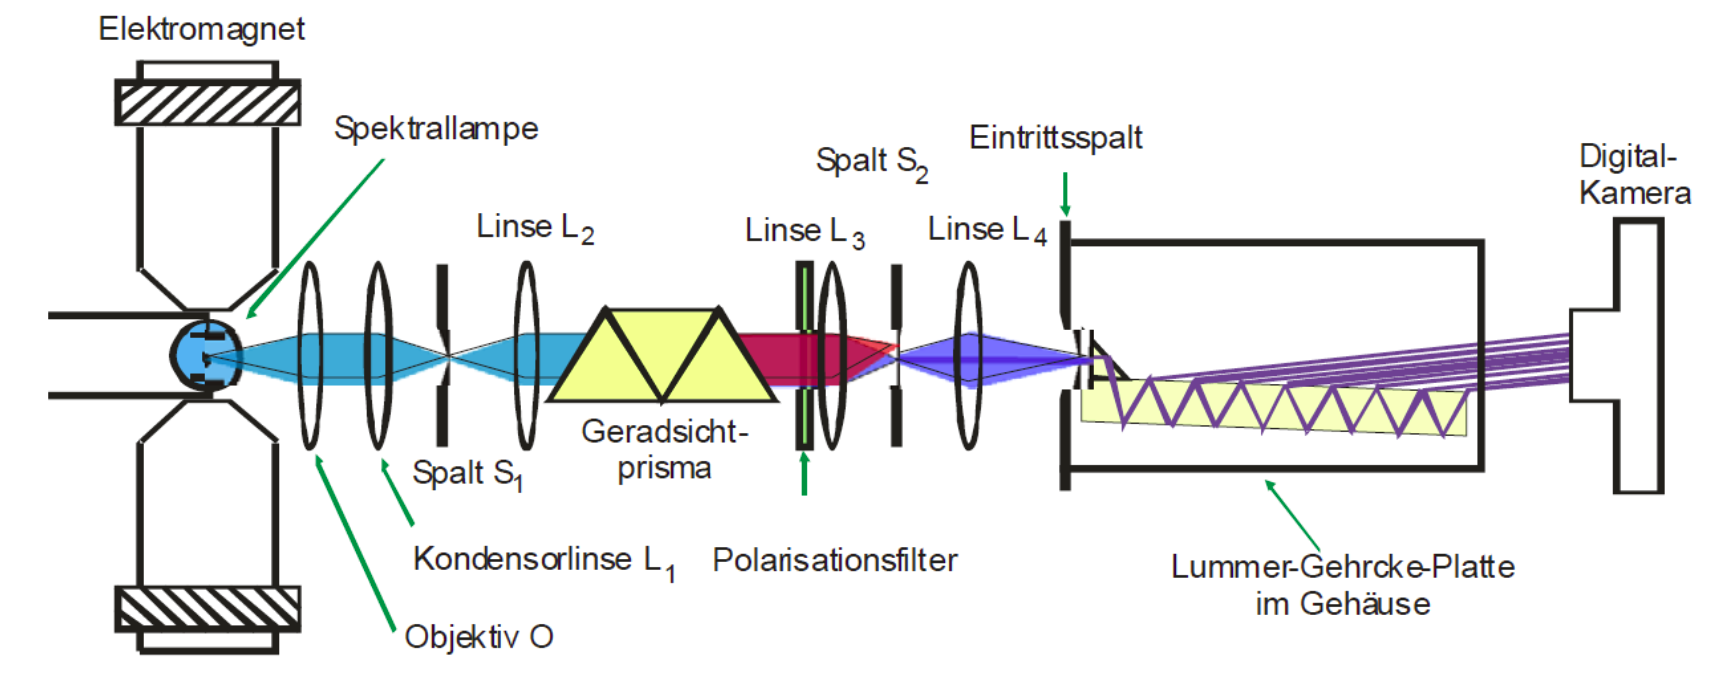
\includegraphics[width=\textwidth]{images/aufbau.png}
  \caption{Fotografie des Versuchsaufbaus. Links ist die Gammastrahlenquelle zu sehen, der Strahlengang zum Detektor durch einen zu untersuchenden Würfel, der gedreht und in den Strahlengang hinein geschoben werden kann, ist eingezeichnet. \cite{Versuchsanleitung}.}
  \label{fig:aufbau}
\end{figure}

Dort ist links die Caesium-Probe, die die Gammastrahlung aussendet, zu sehen. Diese ist abgeschirmt, nur durch eine kleine Blende wird ein Strahl auf den zu untersuchenden Würfel kollimiert. Der Würfel befindet sich auf einer Apparatur, mit der er um seine $z$-Achse wie eingezeichnet gedreht werden kann, außerdem kann er in den Strahlengang herein und herausgedreht werden.

Das Energiespektrum wird mit einem Szintillationsdetektor aufgenommen, der hier durch einen $\ce{NaI}$-Detektor realisiert ist. Durch Streuung an den Atomen im Gitter dieses anorganischen Kristalls regt das einfallende und zu detektierende Gamma-Quant ein oder mehrere Elektronen, Löcher oder Elektronen-Loch-Paare (Exzitonen genannt) an, die sich durch den Kristall weiterbewegen. Dabei wird das Natriumiodid in der Regel mit Thallium dotiert, sodass die Bandstruktur geringfügig geändert wird. Rekombinieren die freigesetzten Teilchen bzw. Quasiteilchen an den sogenannten Aktivatorzentren, also den Fremdatomen, so rekombinieren diese dort und die Atome regen sich unter Aussendung von im Vergleich zu dem einfallenden Photon niederenergetischen Photonen über das sogenannte Aktivatorband ab. Die Photonenenergie ist dann zu niedrig, um ein Elektron vom Valenz- in das Leitungsband zu heben, sodass diese Photonen den Kristall zu einer ersten Photokathode passieren können, wo erste Elektronen ausgelöst werden.
Diese werden danach lawinenartig in einem Photomultiplier mithilfe eines Dynodensystems vervielfältigt. Bei den Dynoden handelt es sich um weitere Photokathoden, auf die die Elektronen mithilfe von elektrischen Feldern beschleunigt werden. Sie sind wegen ihrer Energiezunahme dann selbst in der Lage, weitere Elektronen auszulösen.

Die Impulshöhe des elektrischen Impulses aus den vervielfältigen Elektronen ist dann ein Maß für die Energie des am Anfang eingefallenen Gammaphotons. Um ein Energiespektrum zu erhalten, wird in diesem Versuch ein Multikanalanalysator verwendet. Dieser besteht aus einem Speicher mit einer bestimmten Anzahl an Kanälen. Die Impulshöhe des Signals wird bestimmt und der Speicher des Kanals um eins erhöht, dem die Impulshöhe am nächsten kommt. Dazu muss vorher ein Proportionalitätsfaktor definiert werden, mit dem die Energie in einen Kanal umgerechnet werden kann.
Im Versuch steht ein PC zur Verfügung, mit dem die Spektren digital ausgelesen werden können.

Es werden neben einer Nullmessung von $t=300$\,s vier verschiedene Würfel untersucht. Würfel 1 besteht lediglich aus einem Aluminiumgehäuse, das auch die äußere Schicht der weiteren Würfel bildet. Für diesen Würfel werden drei Projektionen für je $t=120$\,s gemessen. Würfel 2 und Würfel 3, die jeweils vollständig aus einem Material aus der Reihe Aluminium, Blei, Eisen, Messing und Delrin bestehen, werden für vier verschiedene Projektionen für jeweils $t=180$\,s vermessen. Würfel 4 wird für zwölf verschiedene Projektionen für je $t=180$\,s vermessen, seine Elementarwürfel können aus den Materialien aus der obigen Reihe bestehen.

%\section{Fehlerrechnung}
\label{sec:Fehlerrechnung}
Der Mittelwert einer Stichprobe von $N$ Werten wird durch
\begin{equation}
  \overline{x} = \sum\limits_{i = 1}^N x_i
  \label{eqn:mean}
\end{equation}

berechnet.
Die empirische Standardabweichung dieser Stichprobe ist durch
\begin{equation}
  \sigma_x = \sqrt{\frac{1}{N-1}
    \sum\limits_{i = 1}^N
    (x_i-\overline{x})^2}
    \label{eqn:std}
\end{equation}

gegeben.
Ist $f$ eine Funktion, die von unsicheren Variablen $x_i$ mit
Standardabweichungen $\sigma_i$ abhängt, so ist die Unsicherheit von f
\begin{equation}
  \sigma_f = \sqrt{
    \sum\limits_{i = 1}^N
      \left( \frac{\partial f}{\partial x_i} \sigma_i \right)^{\!\! 2}
  }\,.
  \label{eqn:gaussfehler}
\end{equation}

Diese Formel bezeichnet man als "Gauß'sches Fehlerfortpflanzungsgesetz".

Bei einer linearen Regression folgt eine Ausgleichsgerade
\begin{equation}
  y(x) = ax+b\,
\end{equation}
mit der Steigung $a$ und dem Ordinatenabschnitt $b$. Liegen Fehler in y-Richtung
und nur in y-Richtung vor, dann sind die Parameter $a$ und $b$ selbst unsicher
und ergeben sich zu
\begin{align}
  a &= \frac{\overline{xy}-\overline{x} \cdot \overline{y}}{\overline{x^2}-\overline{x}^2}\,,\\
  b &= \frac{\overline{y}-\overline{x^2}-\overline{xy} \cdot \overline{x}}{\overline{x^2}-\overline{x}^2}\,.
\end{align}

%Wenn im Folgenden Mittelwerte, Standardabweichungen und Fehler von
%Funktionen unsicherer Größen berechnet werden, so werden stets die obigen
%Formeln verwendet.
Jegliche Rechnungen werden mit IPython 5.3.0 in Python 3.6.1 durchgeführt. Dabei
werden die Bibliotheken "numpy" \cite{numpy} und "scipy" \cite{scipy} verwendet.
Letztere dient insbesondere zur Erstellung von Ausgleichsrechnungen.
Die Ausführung von Fehlerrechnungen geschieht unter Verwendung des Pakets
"uncertainties" \cite{uncertainties}. Zur Erstellung von Graphen wird die Bibliothek
"matplotlib" \cite{matplotlib} verwendet.

\newpage
\section{Auswertung}
\label{sec:Auswertung}
Im Folgenden werden alle Berechnungen in Python 3.7.1, unterstützt durch das
Paket NumPy \cite{numpy}, durchgeführt. Für die Ausgleichsrechnung wird SciPy
\cite{scipy} verwendet. Die Abbildungen werden mit matplotlib \cite{matplotlib} erstellt.

\subsection{Bestimmung des vertikalen Erdmagnetfeldes}
\label{subsec:vertikal}

Es wurde im Versuch mithilfe eines Helmholtzspulenpaares ein vertikales Magnetfeld
erzeugt, das die vertikale Komponente des Erdmagnetfeldes kompensierte. Die vertikale
Komponente des Erdmagnetfeldes lässt sich daher aus den Daten des Helmholtzspulenpaares
mithilfe der Formel
\begin{equation}
    B= \mu_0 \cdot  \frac{8}{\sqrt {125}}\cdot \frac{I\cdot N}{R}
    \label{eqn:Helmholtz}
\end{equation}
berechnen. Mit den Daten aus der Versuchsanleitung \cite{Versuchsanleitung} und einem Strom von
$I_{\text{vert}}=0{,}195\,$A ergibt sich die vertikale Komponente des Erdmagnetfeldes zu
\begin{equation*}
  \SI{2.99e-5}{\tesla}\,.
\end{equation*}
Der Theoriewert hierzu liegt bei $\SI{44}{\micro\tesla}$ \cite{erde}. Der gemessene Wert
weicht hiervon um $-32{,}05\%$ ab.

\subsection{Bestimmung des horizontalen Erdmagnetfeldes und der Landé-Faktoren}
\label{subsec:horizontal}

Zunächst werden mithilfe von Gleichung \eqref{eqn:Helmholtz} aus den gemessenen Stromstärken
die horizontalen Magnetfeldstärken berechnet. Die gemessenen und die daraus berechneten Werte befinden sich
in Tabelle \ref{tab:werte}.

\begin{table}[htp]
	\begin{center}
    \caption{Messwerte und daraus berechnete Werte für die magnetische Feldstärke.}
    \label{tab:werte}
		\begin{tabular}{ccccc}
		\toprule
			{$f$/kHz} & {$I_1$/A} & {$I_2$/A} & {$B_1$/µT} & {$B_2$/µT}\\
			\midrule
			100 & 0,42 & 0,50 & 25,35 & 30,17\\
			200 & 0,58 & 0,76 & 35,00 & 45,86\\
			300 & 0,76 & 1,00 & 45,86 & 60,35\\
			400 & 0,92 & 1,26 & 55,52 & 76,04\\
			500 & 1,09 & 1,51 & 65,78 & 91,12\\
			600 & 1,26 & 1,76 & 76,04 & 106,21\\
			700 & 1,43 & 2,01 & 86,30 & 121,30\\
			800 & 1,60 & 2,21 & 96,56 & 133,37\\
			900 & 1,76 & 2,52 & 106,21 & 152,08\\
			1000 & 1,93 & 2,77 & 116,47 & 167,16\\
		\bottomrule
		\end{tabular}
	\end{center}
\end{table}

Anschließend wird für beide Isotope getrennt jeweils die horizontale Magnetfeldstärke $B_{\text{hor}}$
gegen die Frequenz $f$ aufgetragen und es wird eine lineare Ausgleichsrechnung der Form
\begin{equation*}
  g(f)=af+b
\end{equation*}
durchgeführt. Es ergeben sich die Parameter
\begin{align*}
 a_1&= \SI{1.0149(0027)e-10}{\tesla\per\Hz}  \,,\\
 b_1&= \SI{1.509(016)e-05}{\tesla} \,,\\
 a_2&= \SI{1.511(012)e-10}{\tesla\per\Hz} \,,\\
 b_2&= \SI{1.53(07)e-05}{\tesla} \,.
\end{align*}
Die zugehörigen Plots sind in den Abbildungen \ref{fig:frequenz1} und \ref{fig:frequenz2} dargestellt.
Es ist erkennbar, dass die Messwerte sich sehr gut durch eine Gerade anpassen lassen.
\begin{figure}
  \centering
  \includegraphics[width=\textwidth]{build/frequenz1.pdf}
  \caption{Messwerte und Ausgleichsrechnung zur Bestimmung des horizontalen B-Feldes und des Landé-Faktors für
  das erste Isotop.}
  \label{fig:frequenz1}
\end{figure}
\begin{figure}
  \centering
  \includegraphics[width=\textwidth]{build/frequenz2.pdf}
  \caption{Messwerte und Ausgleichsrechnung zur Bestimmung des horizontalen B-Feldes und des Landé-Faktors für
  das zweite Isotop.}
  \label{fig:frequenz2}
\end{figure}

Aus den Parametern lassen sich nun die horizontale B-Feldstärke, sowie der Landé-Faktor bestimmen.
Die horizontale Erdmagnetfeldstärke ist gegeben durch den Parameter $b$. Der Theoriewert beträgt hier
$\SI{20}{\micro\tesla}$ \cite{erde}. Die Abweichung vom Theoriewert beträgt damit $-24{,}55\%$ für
$b_1$ und $-23{,}5\%$ für $b_2$.

Der Landé-Faktor kann mithilfe von Gleichung \eqref{eqn:B_M_Theorie} berechnet werden zu
\begin{equation*}
  g_F=\frac{4\pi m_e}{e a} \,.
\end{equation*}
Damit ergeben sich die beiden Werte
\begin{align*}
  g_{F,1}&= \SI{0.7041(0018)}{}\,,\\
  g_{F,2}&= \SI{0.473(004)}{}\,.
\end{align*}
Die Unsicherheiten der $g_{F,i}$ lässt sich durch
\begin{equation}
  \sigma_{g_{F,i}} = \frac{4\pi m_e}{e a_i^2} \sigma_{a_i}
  \label{eqn:sigma_g_F}
\end{equation}
bestimmen \footnote{Ist $f$ eine Funktion, die von unsicheren Variablen $x_i$ mit
Standardabweichungen $\sigma_i$ abhängt, so ist die Unsicherheit von f
\begin{equation}
  \sigma_f = \sqrt{
    \sum\limits_{i = 1}^N
      \left( \frac{\partial f}{\partial x_i} \sigma_i \right)^{\!\! 2}
  }\,.
  \label{eqn:gaussfehler}
\end{equation}
Diese Formel wird auch "Gauß'sches Fehlerfortpflanzungsgesetz" gennant.}.

\subsection{Bestimmung des Kernspins}
\label{subsec:Kernspin}

Für die beiden Rb Isotope gilt $L=0$, $S=\frac{1}{2}$ und $J=\frac{1}{2}$.
Es folgt für Gleichung \eqref{eqn:g_F_Theorie}
\begin{equation*}
  I=\frac{1}{2}\left(\frac{g_J}{g_F}-1\right) \,.
\end{equation*}
Der Landé-Faktor $g_J$ kann mithilfe von Gleichung \eqref{eqn:g_J_Theorie} zu $g_J=2{,}0023$ bestimmt
werden. Für den Kernspin folgt damit
\begin{align*}
  I_1&= \SI{0.922(004)}{}\,,\\
  I_2&= \SI{1.616(017)}{}\,.
\end{align*}
Die Theoriewerte betragen hier $I=5/2$ für $\text{Rb}^{85}$ und $I=3/2$ für $\text{Rb}^{87}$.
Die Unsicherheiten der $I_i$ sind
\begin{equation}
  \sigma_{I_i} = \frac{g_J}{2 g_{F_i}^2} \sigma_{g_{F,i}}\,.
\end{equation}
%mit $\sigma_{g_{F,i}}$ aus Gleichung \eqref{eqn:sigma_g_F}.

Mithilfe des Kernspins können die Isotope wie folgt zugeordnet werden: Isotop 1 ist $\text{Rb}^{87}$
und Isotop 2 ist $\text{Rb}^{85}$. Die Abweichungen von den Theoriewerten betragen
$-35{,}36\%$ für $\text{Rb}^{85}$ und $-38{,}53\%$ für $\text{Rb}^{87}$.


\subsection{Bestimmung des Isotopenverhältnisses}
\label{subsec:Isotope}
In Abbildung \ref{fig:foto} ist ein typischer Verlauf der Transparenz des Rb-Gases in Abhängigkeit
von der magnetischen Feldstärke bei einer Frequenz von $f=100\,$kHz dargestellt.
Aus dem Verhältnis der Tiefen der Dips der beiden
Isotope lässt sich mithilfe von Gleichung \eqref{eqn:transient} das Isotopenverhältnis bestimmen.
Für den ersten Dip ergibt sich eine Amplitude von 4{,}5 Einheiten und für den zweiten
eine Amplitude von 9 Einheiten
\begin{equatio*}
  \frac{\gamma_{85}}{\gamma_{87}}=\frac{9}{4{,}5}= 2 \,.
\end{equation*}

Das in der Natur vorkommende Verhältnis folgt aus den Verhältnissen der beiden Isotope \cite{verhältnis}
und ergibt
\begin{equation*}
  \frac{\text{Anteil}~ \ce{^{85}Rb}}{\text{Anteil}~ \ce{^{87}Rb}}=\frac{72,17\%}{27,83\%} \approx 2{,}593 \,.
\end{equation*}
Der aus den Messwerten berechnete Wert weicht davon um $-22{,}87\%$ ab.

\begin{figure}
  \centering
  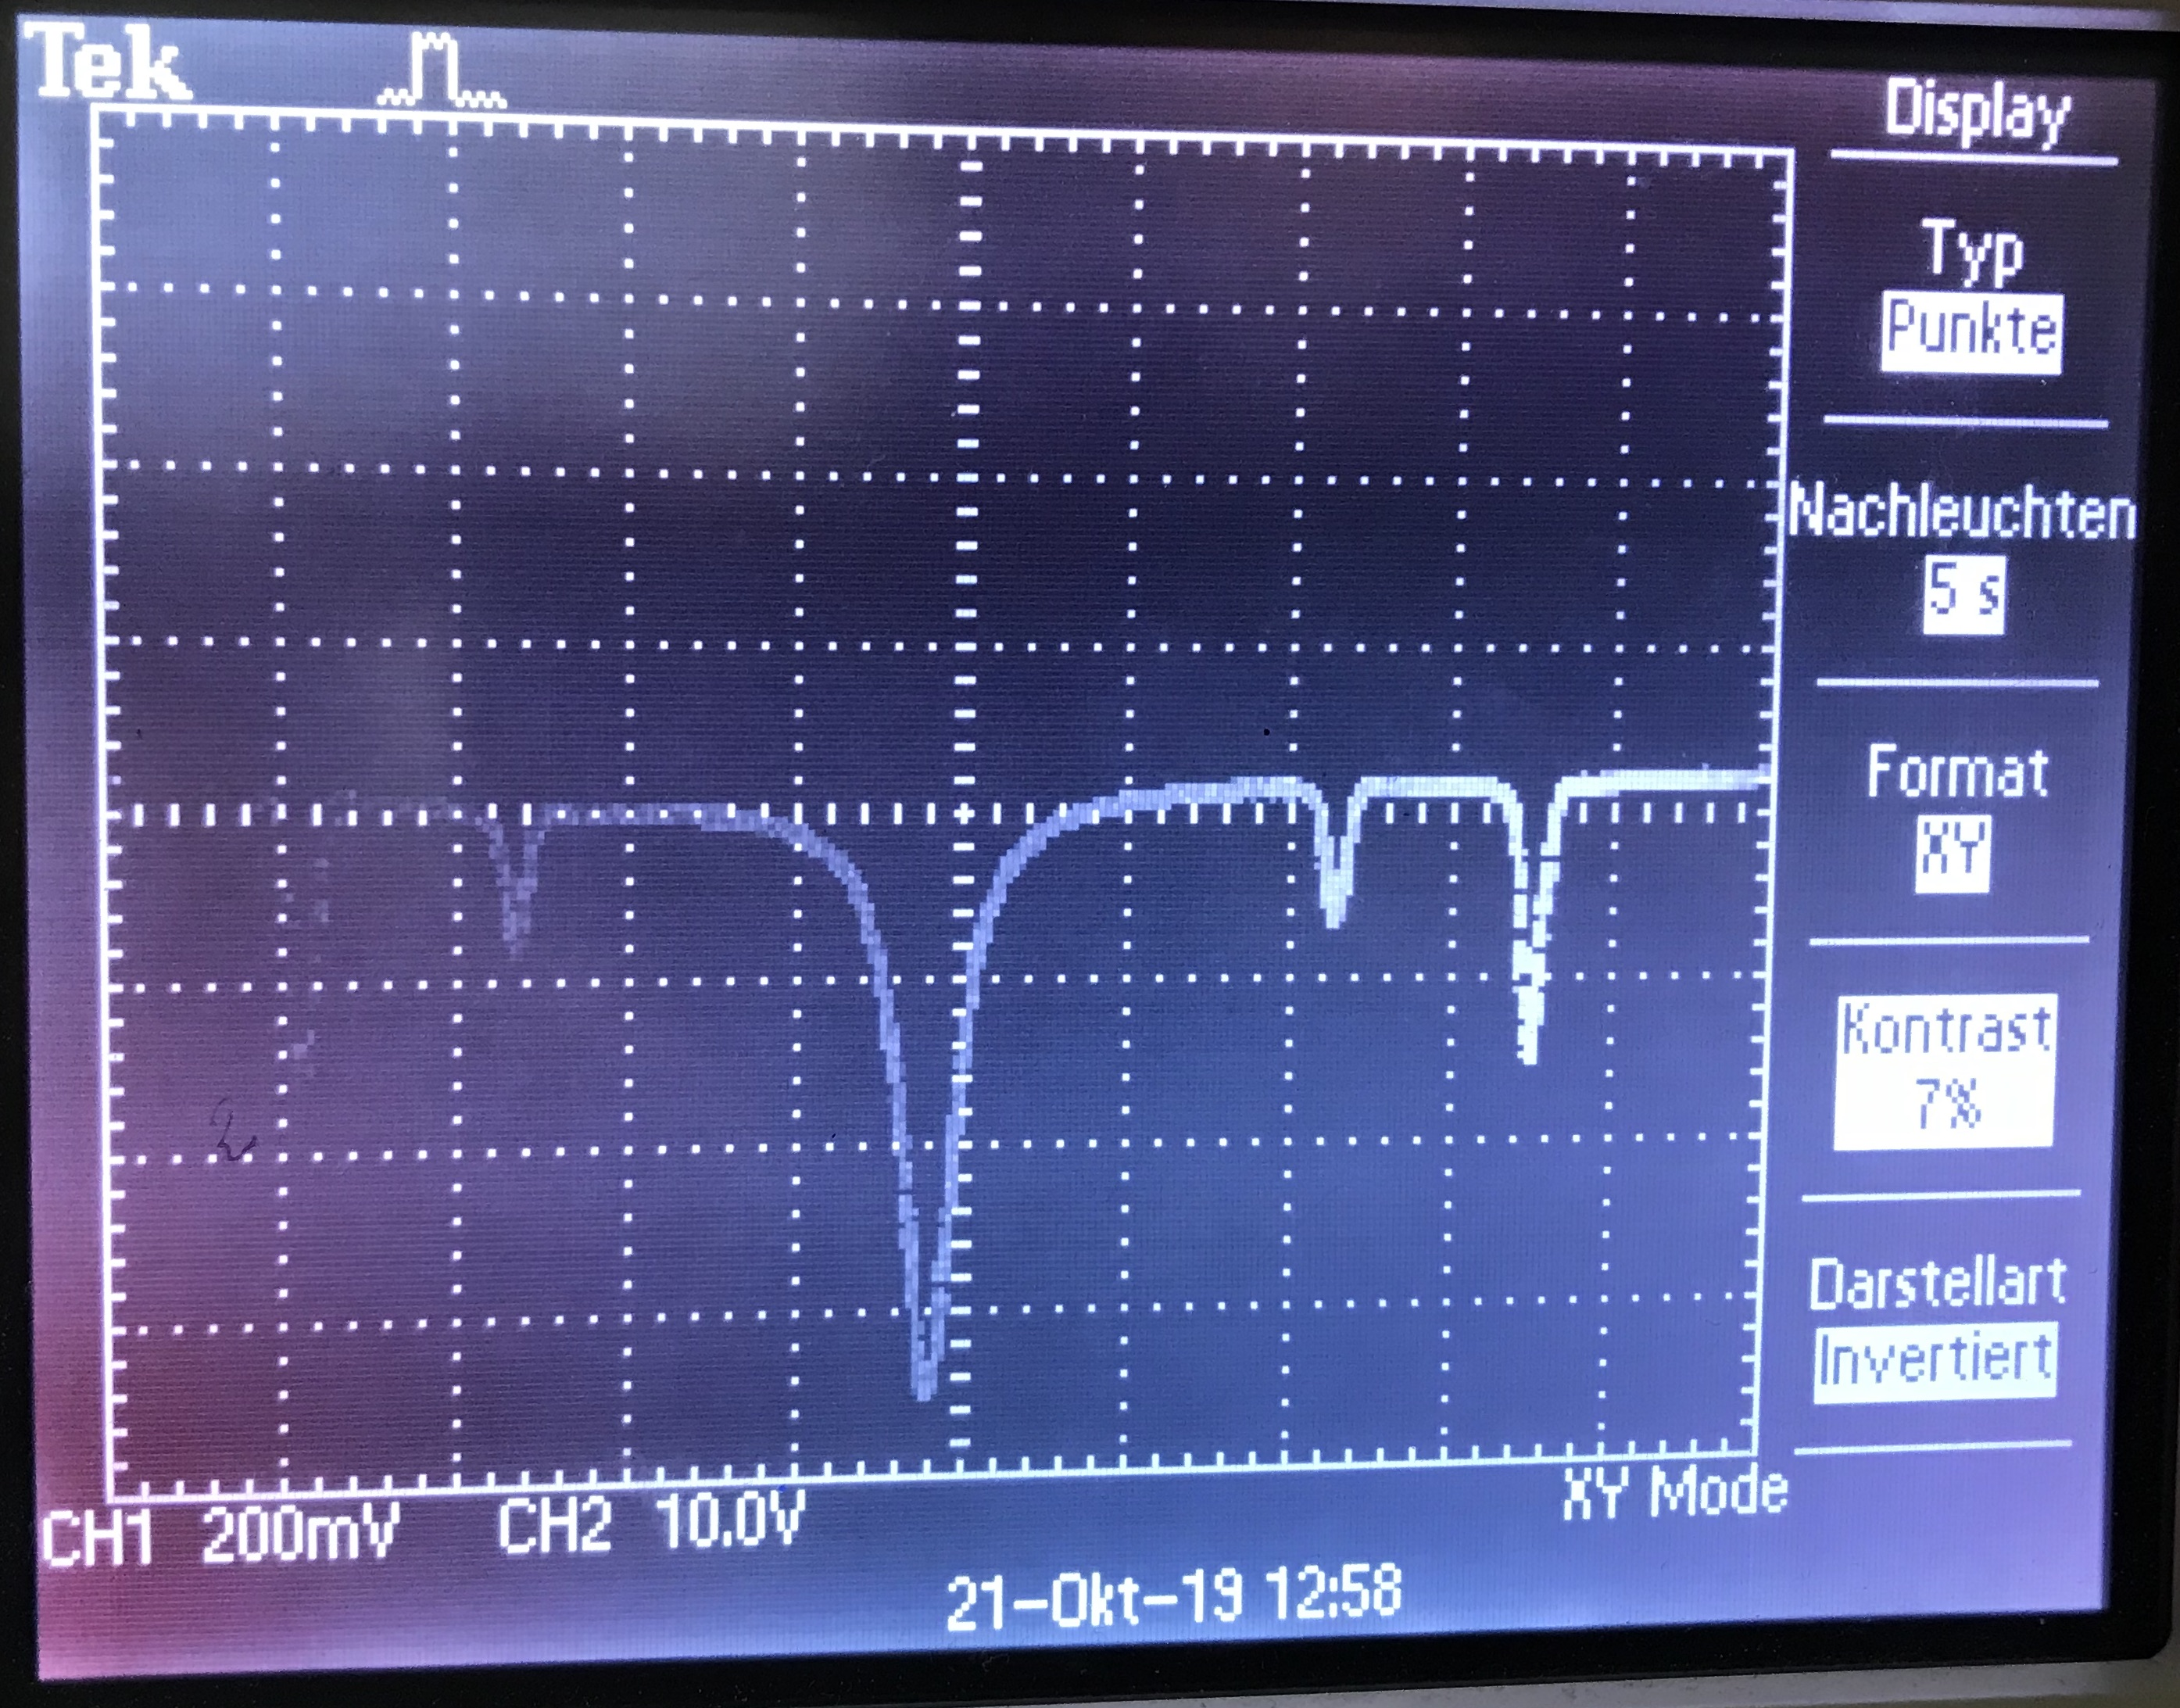
\includegraphics[width=0.7\textwidth]{data/foto.jpg}
  \caption{Typischer Verlauf der Transparenz des Rb-Gases in Abhängigkeit von der magnetischen Feldstärke bei einer Frequenz von $f=100\,$kHz.}
  \label{fig:foto}
\end{figure}


\subsection{Abschätzung des quadratischen Zeeman-Effekts}
\label{subsec:zeeman}
In diesem Kapitel soll abgeschätzt werden, wie groß der Einfluss des quadratischen Zeeman-Effekts
in diesem Versuch ist. Der quadratische Zeeman-Effekt kann durch Gleichung
\eqref{eqn:zeemanDifferenzQuadratisch} beschrieben werden. Gemäß der Versuchsanleitung \cite{Versuchsanleitung} beträgt die
Hyperfeinstrukturaufspaltung des Grundzustandes
\begin{align*}
  \Delta E_{85}&= \SI{2.01e-24}{\joule}\,,\\
  \Delta E_{87}&= \SI{4.53e-24}{\joule}\,.
\end{align*}
Mit den jeweiligen berechneten Werten $B_i$ für die Horizontalkomponente des Erdmagnetfeldes,
$g_{F,i}$ für die Landé-Faktoren und $M_F=1$ ergibt sich damit für den quadratischen Zeeman-Effekt
\begin{align*}
  \Delta E_{Z,85}&=\SI{6.7(4)e-29}{\joule}\,,\\
  \Delta E_{Z,87}&=\SI{9.85(13)e-29}{\joule}\,.
\end{align*}
Die Unsicherheiten der $\Delta E_{Z,i}$ betragen
\begin{equation}
  \sigma_{\Delta E_{Z,i}} = \left( \mu_{\text{B}} B + 2 g_{F,i} \mu_{\text{B}}^2 B^2 \frac{1 - 2 M_F}{\Delta E_{\text{Hy}}} \right) \sigma_{g_{F,i}}\,.
  \label{eqn:sigma_Delta_E_Z}
\end{equation}

Die zusätzlich zum linearen Zeeman-Effekt durch den quadratischen Term herbeigeführte Aufspaltung beträgt dabei lediglich
\begin{align*}
  \Delta E_{\text{quadratisch},85}&=\SI{-2.24(25)e-33}{\joule}\,,\\
  \Delta E_{\text{quadratisch},87}&=\SI{-2.14(06)e-33}{\joule}\,,
\end{align*}
wobei die Unsicherheiten durch den zweiten Term in Gleichung \eqref{eqn:sigma_Delta_E_Z} beschrieben werden.
Somit ist der quadratische Zeeman-Effekt in diesem Versuch vernachlässigbar.

\subsection{Anpassung der ansteigenden Flanken an eine Exponentialfunktion}
\label{subsec:flanken}

In diesem Kapitel sollen die ansteigenden Flanken aus dem letzten Versuchsteil an
Exponentialfunktionen angepasst werden. Dafür werden zunächst Werte aus den angefertigten
Bildern abgelesen. Die Aufnahmen des Oszilloskops befinden sich in den Abbildungen
\ref{fig:flanke1} und \ref{fig:flanke2}. Die daraus abgelesenen Werte befinden sich in
Tabelle \ref{tab:flanke}.

\begin{figure}
  \centering
  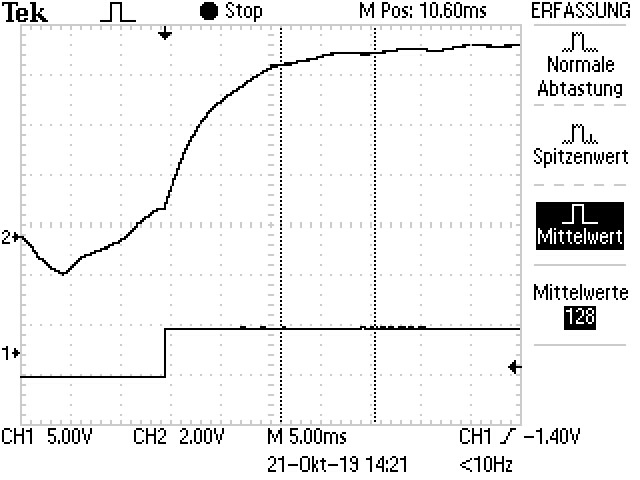
\includegraphics[width=0.7\textwidth]{data/Dip1.jpg}
  \caption{Ansteigende Flanke für den ersten Dip.}
  \label{fig:flanke1}
\end{figure}
\begin{figure}
  \centering
  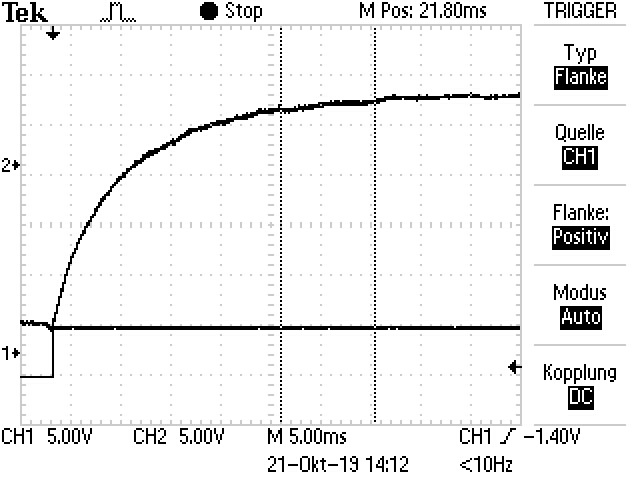
\includegraphics[width=0.7\textwidth]{data/Dip2.jpg}
  \caption{Ansteigende Flanke für den zweiten Dip.}
  \label{fig:flanke2}
\end{figure}

\begin{table}[htp]
	\begin{center}
    \caption{Aus den Bildern abgelesene und auf 1 normierte Werte für die Transparenz in Abhängigkeit von der Zeit.}
    \label{tab:flanke}
		\begin{tabular}{cccc}
		\toprule
			{$t_1$/ms} & {$\text{Transparenz}_1$} & {$t_2$/ms} & {$\text{Transparenz}_2$}\\
			\midrule
			22,5 & 0,09 & 15,0 & 0,00\\
			25,0 & 0,23 & 20,0 & 0,18\\
			30,0 & 0,34 & 25,0 & 0,29\\
			35,0 & 0,51 & 30,0 & 0,40\\
			40,0 & 0,57 & 35,0 & 0,49\\
			45,0 & 0,66 & 40,0 & 0,56\\
			50,0 & 0,69 & 45,0 & 0,62\\
			55,0 & 0,74 & 50,0 & 0,67\\
			60,0 & 0,77 & 55,0 & 0,71\\
			65,0 & 0,80 & 60,0 & 0,73\\
			70,0 & 0,86 & 65,0 & 0,76\\
			75,0 & 0,91 & 70,0 & 0,78\\
			80,0 & 0,91 & 75,0 & 0,80\\
			85,0 & 0,94 & 80,0 & 0,82\\
			90,0 & 0,94 & 85,0 & 0,84\\
			95,0 & 0,97 & 90,0 & 0,87\\
			100 & 0,97 & 95,0 & 0,89\\
			105 & 0,97 & 100 & 0,91\\
			110 & 0,97 & 105 & 0,91\\
			115 & 0,97 & 110 & 0,93\\
			120 & 0,97 & 115 & 0,93\\
			125 & 0,97 & 120 & 0,96\\
			130 & 0,97 & 125 & 0,96\\
			135 & 1,00 & 130 & 0,96\\
			140 & 1,00 & 135 & 0,96\\
			145 & 1,00 & 140 & 0,98\\
			150 & 1,00 & 145 & 0,98\\
			- & - & 150 & 0,98\\
			- & - & 155 & 1,00\\
			- & - & 160 & 1,00\\
			- & - & 165 & 1,00\\
			- & - & 170 & 1,00\\
			- & - & 175 & 1,00\\
			- & - & 180 & 1,00\\
			- & - & 185 & 1,00\\
			- & - & 190 & 1,00\\
		\bottomrule
		\end{tabular}
	\end{center}
\end{table}

Die Werte werden auf 1 normiert. Anschließend wird eine Ausgleichsrechnung der Form
\begin{equation*}
  f(t)=1-\exp(-a(t-b))
\end{equation*}
durchgeführt. Es ergeben sich die Parameter
\begin{align*}
  a_1&=\SI{0.0398(0010)}{\per\milli\second} \,,\\
  b_1&=\SI{19.2(4)}{\milli\second} \,,\\
  a_2&=\SI{0.0285(0005)}{\per\milli\second}\,,\\
  b_2&=\SI{13.3(5)}{\milli\second} \,.
\end{align*}
In den Abbildungen \ref{fig:flankefit1} und \ref{fig:flankefit2} sind die Messwerte und die
Ausgleichsrechnungen grafisch dargestellt. Es ist erkennbar, dass sich die Messwerte gut
durch eine Exponentialfunktion annähern lassen.

\begin{figure}
  \centering
  \includegraphics[width=\textwidth]{build/flanke1.pdf}
  \caption{Messwerte und Ausgleichsfunktion für den ersten Dip.}
  \label{fig:flankefit1}
\end{figure}
\begin{figure}
  \centering
  \includegraphics[width=\textwidth]{build/flanke2.pdf}
  \caption{Messwerte und Ausgleichsfunktion für den zweiten Dip.}
  \label{fig:flankefit2}
\end{figure}

\newpage
\subsection{Bestimmung des Verhältnisses der Landé-Faktoren mithilfe der Rabi-Oszillationen}
\label{subsec:oszillationen}
Zur Bestimmung des Verhältnisses der Landé-Faktoren mithilfe der Rabi-Oszillationen werden
die gemessenen Periodendauern der Oszillationen gegen die Amplitude des RF-Feldes aufgetragen.
Die zugehörigen Messwerte befinden sich in Tabelle \ref{tab:oszi}.

\begin{table}[htp]
	\begin{center}
    \caption{Messwerte für die Periodendauern der Oszillationen in Abhängigkeit von der Amplitude des RF-Feldes.}
    \label{tab:oszi}
		\begin{tabular}{ccc}
		\toprule
			{$U$/V} & {$T_1$/ms} & {$T_2$/ms}\\
			\midrule
			2 & 1,50 & 2,52\\
			3 & 1,16 & 1,84\\
			4 & 0,89 & 1,29\\
			5 & 0,71 & 1,07\\
			6 & 0,61 & 0,90\\
			7 & 0,51 & 0,77\\
			8 & 0,45 & 0,67\\
			9 & 0,40 & 0,60\\
			10& 0,36 & 0,54\\
		\bottomrule
		\end{tabular}
	\end{center}
\end{table}

Außerdem wird eine Ausgleichsrechnung der Form
\begin{equation*}
  f(x)=a+\frac{b}{x-c}
\end{equation*}
durchgeführt. Dies ist in den Abbildungen \ref{fig:oszi1} und \ref{fig:oszi2} grafisch dargestellt.
Es ergeben sich die Parameter
\begin{align*}
  a_1&=\SI{-0.14(4)e-3}{\second} \,,\\
  b_1&=\SI{5.5(5)e-3}{\volt} \,,\\
  c_1&=\SI{-1.34(24)}{\volt} \,,\\
  a_2&=\SI{-7(8)e-05}{\second} \,,\\
  b_2&=\SI{6.2(7)e-3}{\volt} \,,\\
  c_2&=\SI{-0.39(22)}{\volt} \,.
\end{align*}
Das Verhältnis der Parameter $b_i$ für $\text{Rb}^{85}$ und $\text{Rb}^{87}$ beträgt damit:
\begin{equation*}
  \frac{b_2}{b_1}\approx\SI{1.13(17)}{}\,
\end{equation*}
mit der Unsicherheit
\begin{equation}
  \sigma_{b_2/b_1} = \sqrt{\left( \frac{1}{b_1}\sigma_{b_2} \right)^2 + \left( \frac{b_2}{b_1^2} \sigma_{b_1} \right)^2}
\end{equation}
Dieser Wert weicht um $-24{,}67\%$ vom Theoriewert 1{,}5 ab.
\begin{figure}
  \centering
  \includegraphics[width=\textwidth]{build/oszi1.pdf}
  \caption{Messwerte und Ausgleichsrechnung zur Bestimmung des Verhältnisses der Landé-Faktoren mithilfe der
  Rabi-Oszillationen für $\text{Rb}^{87}$.}
  \label{fig:oszi1}
\end{figure}
\begin{figure}
  \centering
  \includegraphics[width=\textwidth]{build/oszi2.pdf}
  \caption{Messwerte und Ausgleichsrechnung zur Bestimmung des Verhältnisses der Landé-Faktoren mithilfe der
  Rabi-Oszillationen für $\text{Rb}^{85}$.}
  \label{fig:oszi2}
\end{figure}

\section{Diskussion}
\label{sec:Diskussion}

Zusammenfassend lässt sich der Versuch nur bedingt als erfolgreich bewerten.

Im Spektrum ist ein eindeutiger Peak Peak zu sehen. Außerdem ist ein Compton-Spektrum
zu sehen, das aus der Wechselwirkung der Gammaphotonen mit dem Szintillator entsteht.

Die gemessenen Zählraten für die Nullmessung mit einem hohlen Aluminiummantel
ergeben sich zu
\begin{align*}
  I_0,1&=\SI{171.83(135)}{\per\second} \,, \\
  I_0,2&=\SI{169.63(133)}{\per\second} \,, \\
  I_0,3&=\SI{158.78(133)}{\per\second} \,.
\end{align*}

Für die Absorptionskoeffizienten der beiden homogenen Würfel ergibt sich unter Verwendung der
Werte für den hohlen Aluminiummantel
\begin{align*}
  \bar{\mu_2}&= \SI{0.614(42)}{1\per \centi\metre}\,, \\
  \bar{\mu_3}&=\SI{0.133(9)}{1\per \centi\metre} \,.
\end{align*}
Damit wird das Material in Würfel 2 zu Messing mit einer Abweichung von $1{,}57\%$
und das in Würfel 3 zu CH2O mit einer Abweichung von $14{,}75\%$ bestimmt. Es liegt
jedoch keine Information darüber vor, aus welchen Materialien die Würfel tatsächlich bestehen.
Es ist zudem anzumerken, dass der statistische Fehler in diesem Rechenschritt recht groß
wird, da die Nullmessungen für den hohlen Aluminiummantel nur 120\,s lang waren.

Die bestimmten Materialien des zusammengesetzten Würfels sind in Tabelle \ref{tab:ergebnisse2}
aufgeführt.

(UND DANN HIER NOCH WAS MAN DA SO ERKENNEN KANN...)

\newpage
\addsec{Anhang}
\label{sec:Anhang}

\begin{figure}[h!]
  \centering
  
\includegraphics[width=0.85\textwidth]{data/temp/rot_ohneB_0.JPG}
  \caption{\cite{insert Beschriftung}.}
  \label{fig:rotOhneB0}
\end{figure}
\begin{figure}[h!]
  \centering
  
\includegraphics[width=0.95\textwidth]{data/temp/rot_mitB_0.JPG}
  \caption{\cite{insert Beschriftung 2}}
  \label{fig:rotMitB0}
\end{figure}

\begin{figure}[h!]
  \centering
  
\includegraphics[width=0.85\textwidth]{data/temp/rot_ohneB_0_aufgehellt.JPG}
  \caption{\cite{insert Beschriftung 3}.}
  \label{fig:rotOhneB0_aufgehellt}
\end{figure}
\begin{figure}[h!]
  \centering
  
\includegraphics[width=0.95\textwidth]{data/temp/rot_mitB_0_aufgehellt.JPG}
  \caption{\cite{insert Beschriftung 4}}
  \label{fig:rotMitB0_aufgehellt}
\end{figure}


\begin{figure}[h!]
  \centering
  
\includegraphics[width=0.85\textwidth]{data/temp/rot_ohneB_90.JPG}
  \caption{\cite{insert Beschriftung 5}.}
  \label{fig:roteOhneB90}
\end{figure}
\begin{figure}[h!]
  \centering
  
\includegraphics[width=0.95\textwidth]{data/temp/rot_mitB_90.JPG}
  \caption{\cite{insert Beschriftung 6}}
  \label{fig:rotMitB90}
\end{figure}

\begin{figure}[h!]
  \centering
  
\includegraphics[width=0.85\textwidth]{data/temp/rot_ohneB_90_aufgehellt.JPG}
  \caption{\cite{insert Beschriftung 7}.}
  \label{fig:roteOhneB90_aufgehellt}
\end{figure}
\begin{figure}[h!]
  \centering
  
\includegraphics[width=0.95\textwidth]{data/temp/rot_mitB_90_aufgehellt.JPG}
  \caption{\cite{insert Beschriftung 8}}
  \label{fig:rotMitB90_aufgehellt}
\end{figure}



\begin{figure}[h!]
  \centering
  
\includegraphics[width=0.85\textwidth]{data/temp/blau_ohneB_0.JPG}
  \caption{\cite{insert Beschriftung 9}.}
  \label{fig:blauOhneB0}
\end{figure}
\begin{figure}[h!]
  \centering
  
\includegraphics[width=0.95\textwidth]{data/temp/blau_mitB_0.JPG}
  \caption{\cite{insert Beschriftung 10}}
  \label{fig:blauMitB0}
\end{figure}

\begin{figure}[h!]
  \centering
  
\includegraphics[width=0.85\textwidth]{data/temp/blau_ohneB_90.JPG}
  \caption{\cite{insert Beschriftung 11}.}
  \label{fig:blauOhneB90}
\end{figure}
\begin{figure}[h!]
  \centering
  
\includegraphics[width=0.95\textwidth]{data/temp/blau_mitB_90.JPG}
  \caption{\cite{insert Beschriftung 12}}
  \label{fig:blauMitB90}
\end{figure}


\newpage
\printbibliography

\end{document}
